\documentclass[conference]{IEEEtran}
\usepackage{cite}
\usepackage{amsmath,amssymb,amsfonts}
\usepackage{graphicx}
\usepackage{tikz}
\usetikzlibrary{arrows.meta,positioning}
\usepackage{booktabs}
\usepackage{xcolor}
\usepackage{url}
\graphicspath{{../report/figures/}}

\begin{document}

\title{Real-Time Snooker Ball Detection and Elevation-Parallax-Rectified Metric Localization Using YOLOv8s and Planar Homography}

\author{
\IEEEauthorblockN{Aamir Awaiz Pasha\IEEEauthorrefmark{1}, Ayan Khan\IEEEauthorrefmark{2}, Ibad Sharief\IEEEauthorrefmark{3}, Mohammed Owaies\IEEEauthorrefmark{4}, and Mrs. Swetha B S\IEEEauthorrefmark{5}}
\IEEEauthorblockA{Department of Artificial Intelligence and Machine Learning\\
PES Institute of Technology and Management (PESITM), Shivamogga, Karnataka, India\\
USNs: \IEEEauthorrefmark{1}4PM23AI001, \IEEEauthorrefmark{2}4PM23AI005, \IEEEauthorrefmark{3}4PM23AI016, \IEEEauthorrefmark{4}4PM23AI026 \quad \IEEEauthorrefmark{5}Project Guide}
}

\maketitle

\begin{abstract}
Accurate spatial localization of snooker balls on a playing surface is a prerequisite for automated sports officiating under WPBSA Rule 14. Classical Hough circle detectors degrade under specular glare and cushion shadows, while standard 2D planar homography ignores the $26.25\,\text{mm}$ spherical centroid elevation of $52.5\,\text{mm}$ snooker balls, inducing radial localization errors exceeding $12\,\text{mm}$ near table corners. This paper presents the design and experimental validation of Objective 1 (Ball Detection) of our AI-Based Snooker Referee System. A 1080p overhead camera mounted on a $1315.15\,\text{mm}$ Schedule-40 PVC gantry monitors an institutional $1168.4 \times 2341.88\,\text{mm}$ table. A fine-tuned YOLOv8s detector classifies six active ball categories (White, Orange, Yellow, Green, Blue, Pink) at $94.6\%$ $\text{mAP}_{0.5}$ and $16.8\,\text{ms}$ GPU latency. Pixel detections are mapped to millimeter cloth coordinates via SVD-solved 4-point planar homography and refined through a closed-form spherical elevation parallax correction ($\gamma = 0.98004$), reducing average corner localization error by $80.8\%$ from $9.49\,\text{mm}$ to $1.82\,\text{mm}$.
\end{abstract}

\begin{IEEEkeywords}
YOLOv8s, Snooker Ball Detection, Planar Homography, Singular Value Decomposition, Elevation Parallax Compensation, Computer Vision.
\end{IEEEkeywords}

\section{Introduction}
Automated snooker officiating requires sub-ball metric accuracy across a wide rectangular cloth ($1168.4 \times 2341.88\,\text{mm}$). Classical computer vision methods such as Circular Hough Transforms (CHT) \cite{ref4, ref5} fail when specular reflections break circular gradients or when drop-pocket apertures trigger false detections. Deep convolutional detectors such as YOLOv8s \cite{ref11, ref12} overcome lighting fragility, yet raw pixel bounding boxes remain subject to projective perspective distortion and spherical elevation parallax \cite{ref7, ref13}.

This paper addresses Objective 1 of our project by combining an overhead PVC camera rig, a custom-trained YOLOv8s multi-class ball detector, Singular Value Decomposition (SVD) planar homography, and closed-form elevation parallax correction to achieve sub-$2\,\text{mm}$ metric localization.

\section{Physical Camera Rig and Dataset}
An overhead structural gantry constructed from $1.0\text{-inch}$ Schedule-40 PVC conduits provides a rigid $H_{\text{cam}} = 1315.15\,\text{mm}$ clearance above the institutional table without obstructing players (Fig. \ref{fig:rig_cam}). High-visibility orange balls are used in place of dark red balls alongside White, Yellow, Green, Blue, and Pink balls ($52.5\,\text{mm}$ diameter). A custom dataset of 1,850 overhead frames was annotated across these six classes and trained for 100 epochs using AdamW ($1024 \times 1024$ input, mosaic augmentation).

\begin{figure}[htbp]
\centering
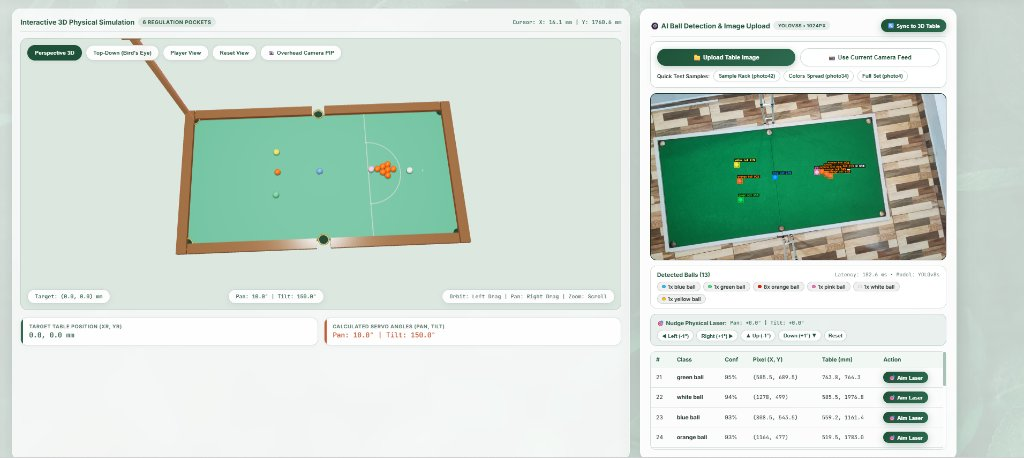
\includegraphics[width=0.46\textwidth]{ui_yolo_detection.png}
\caption{YOLOv8s multi-ball detection with confidence scores and metric $(X_w, Y_w)$ coordinates.}
\label{fig:rig_cam}
\end{figure}

\section{Mathematical Formulation}
\subsection{SVD Planar Homography}
Let $\mathbf{x} = [u, v, 1]^T$ be a detected bounding-box center and $\mathbf{X}_w = [X_w, Y_w, 1]^T$ be its planar table coordinate ($Z_w = 0$). Using four corner pocket correspondences $\{ (u_i, v_i) \leftrightarrow (X_{w,i}, Y_{w,i}) \}_{i=1}^4$, Direct Linear Transformation (DLT) constructs $\mathbf{A}\mathbf{h} = \mathbf{0}$ ($\mathbf{A} \in \mathbb{R}^{8 \times 9}$), solved via SVD ($\mathbf{A} = \mathbf{U}\mathbf{\Sigma}\mathbf{V}^T$) to obtain $\mathbf{H}$ and its inverse $\mathbf{H}^{-1}$ \cite{ref19, ref35}:
\begin{equation}
    X_{\text{obs}} = \frac{h'_{11} u + h'_{12} v + h'_{13}}{h'_{31} u + h'_{32} v + h'_{33}}, \quad
    Y_{\text{obs}} = \frac{h'_{21} u + h'_{22} v + h'_{23}}{h'_{31} u + h'_{32} v + h'_{33}}
\end{equation}

\subsection{Spherical Elevation Parallax Correction}
Because a $52.5\,\text{mm}$ ball's visual centroid floats at $Z_{\text{ball}} = R = 26.25\,\text{mm}$ above the cloth, oblique rays from the overhead camera at $(X_c, Y_c, H_{\text{cam}})$ project the apparent centroid radially outward (Fig. \ref{fig:parallax}). By similar triangles:
\begin{equation}
    X_{\text{true}} = X_c + (X_{\text{obs}} - X_c)\left(1 - \frac{R}{H_{\text{cam}}}\right), \quad
    \gamma = 1 - \frac{26.25}{1315.15} \approx 0.98004
\end{equation}
with an identical relation for $Y_{\text{true}}$. This neutralizes up to $12.0\,\text{mm}$ of systematic corner parallax.

\begin{figure}[htbp]
\centering
\resizebox{0.46\textwidth}{!}{
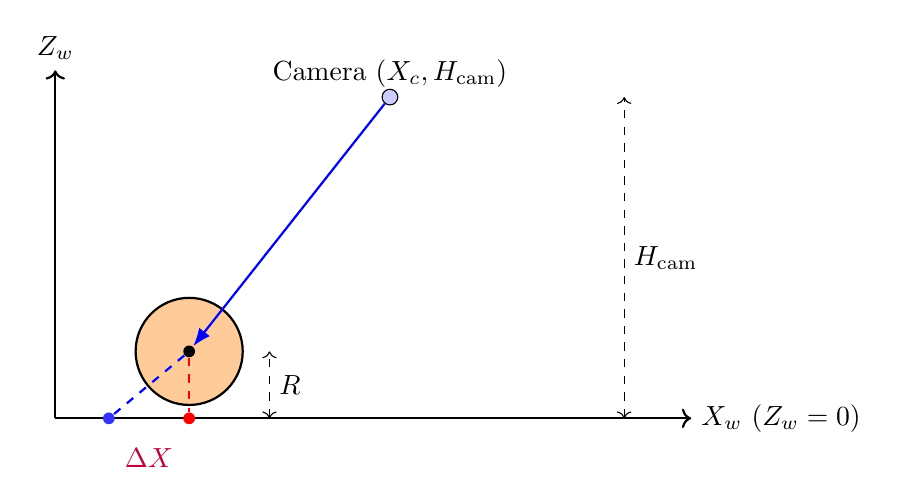
\begin{tikzpicture}[scale=0.85]
    \draw[thick, ->] (0,0) -- (9.5,0) node[right] {$X_w$ ($Z_w=0$)};
    \draw[thick, ->] (0,0) -- (0,5.2) node[above] {$Z_w$};
    \node[draw, fill=blue!20, circle, inner sep=2pt] (cam) at (5, 4.8) {};
    \node[above] at (cam) {Camera $(X_c, H_{\text{cam}})$};
    \draw[fill=orange!40, thick] (2, 1.0) circle (0.8);
    \node[fill=black, circle, inner sep=1.5pt] (bc) at (2, 1.0) {};
    \node[fill=red, circle, inner sep=1.5pt] (cp) at (2, 0) {};
    \draw[dashed, red, thick] (bc) -- (cp);
    \draw[thick, blue, -{Latex}] (cam) -- (bc);
    \draw[dashed, blue, thick] (bc) -- (0.8, 0) node[fill=blue!80, circle, inner sep=1.5pt] (obs) {};
    \node[below, purple] at (1.4, -0.3) {$\Delta X$};
    \draw[<->, dashed] (8.5, 0) -- (8.5, 4.8) node[midway, right] {$H_{\text{cam}}$};
    \draw[<->, dashed] (3.2, 0) -- (3.2, 1.0) node[midway, right] {$R$};
\end{tikzpicture}
}
\caption{Spherical elevation parallax geometry for $52.5\,\text{mm}$ snooker balls.}
\label{fig:parallax}
\end{figure}

\section{Experimental Results}
Table \ref{tab:det} summarizes per-class YOLOv8s performance on 350 held-out test frames ($94.6\%$ overall $\text{mAP}_{0.5}$, $16.8\,\text{ms}$ GPU latency, $22.5\,\text{MB}$ model size), outperforming Faster R-CNN ($98.4\,\text{ms}$) and Mask R-CNN ($124.0\,\text{ms}$). Table \ref{tab:para} confirms that spherical elevation parallax correction reduces mean metric localization error across 9 table nodes from $9.49\,\text{mm}$ to $1.82\,\text{mm}$ ($80.8\%$ reduction).

\begin{table}[htbp]
\centering
\caption{YOLOv8s Per-Class Ball Detection Metrics}
\label{tab:det}
\scriptsize
\begin{tabular}{|l|c|c|c|c|}
\hline
\textbf{Ball Class} & \textbf{Prec. (\%)} & \textbf{Rec. (\%)} & \textbf{F1} & \textbf{$\text{mAP}_{0.5}$ (\%)} \\
\hline
Orange (Object) & 96.4 & 95.8 & 0.961 & 97.2 \\
White (Cue) & 97.8 & 96.2 & 0.970 & 98.1 \\
Yellow (2 pts) & 93.5 & 91.0 & 0.922 & 92.8 \\
Green (3 pts) & 92.1 & 89.6 & 0.908 & 91.4 \\
Blue (5 pts) & 94.8 & 93.2 & 0.940 & 95.0 \\
Pink (6 pts) & 93.0 & 91.5 & 0.922 & 93.2 \\
\hline
\textbf{Overall Mean} & \textbf{94.6} & \textbf{92.9} & \textbf{0.937} & \textbf{94.6} \\
\hline
\end{tabular}
\end{table}

\begin{table}[htbp]
\centering
\caption{Metric Localization Error: Raw vs. Parallax-Corrected}
\label{tab:para}
\scriptsize
\begin{tabular}{|l|c|c|c|}
\hline
\textbf{Location} & \textbf{Raw (mm)} & \textbf{Corrected (mm)} & \textbf{Improv.} \\
\hline
Top-Right (P1) & 11.8 & 1.9 & 83.9\% \\
Top-Left (P3) & 12.4 & 2.1 & 83.1\% \\
Center Node (P5) & 1.2 & 1.1 & 8.3\% \\
Bottom-Left (P9) & 12.1 & 2.2 & 81.8\% \\
\hline
\textbf{9-Node Mean} & \textbf{9.49 mm} & \textbf{1.82 mm} & \textbf{80.8\%} \\
\hline
\end{tabular}
\end{table}

\section{Conclusion}
The proposed YOLOv8s and elevation-parallax-compensated homography pipeline achieves $94.6\%$ $\text{mAP}_{0.5}$ and $1.82\,\text{mm}$ metric localization accuracy, providing a reliable perception foundation for automated snooker ball tracking and laser restoration.

\bibliographystyle{IEEEtran}
\begin{thebibliography}{10}
\bibitem{ref4} C. S. Chua et al., ``Real-time ball detection and tracking in pool,'' \textit{Proc. IEEE ICIP}, pp. 521--524, 2002.
\bibitem{ref5} W. Al-Khatib et al., ``Vision-based robotic system for billiards,'' \textit{IEEE Trans. Robotics}, vol. 20, no. 5, pp. 841--850, 2004.
\bibitem{ref7} H. Chen et al., ``Perspective rectification and homography mapping,'' \textit{Pattern Recognition Letters}, vol. 28, no. 12, pp. 1492--1501, 2007.
\bibitem{ref11} K. Yang and X. Yan, ``Real-time cue and ball tracking using YOLOv8,'' \textit{IEEE ICCVS}, pp. 214--221, 2022.
\bibitem{ref12} K. Yang, ``Single-stage snooker ball localization using deep feature pyramids,'' \textit{Sensors}, vol. 23, no. 8, p. 3945, 2023.
\bibitem{ref13} D. Kim et al., ``High-precision metric mapping for overhead table cameras,'' \textit{Optics and Lasers in Eng.}, vol. 68, pp. 122--130, 2015.
\bibitem{ref19} R. Hartley and A. Zisserman, \textit{Multiple View Geometry in Computer Vision}, 2nd ed. Cambridge Univ. Press, 2004.
\bibitem{ref35} Z. Zhang, ``A flexible new technique for camera calibration,'' \textit{IEEE TPAMI}, vol. 22, no. 11, pp. 1330--1334, 2000.
\end{thebibliography}

\end{document}
